%!TEX root = ../EmbSW2.tex
\section{Embedded Security}

\subsection{Goals and Non-Goals}
\begin{multicols}{2}
  Goals:
  \begin{itemize}
    \item Developing Secure Embedded Systems
    \item Designing Security into Embedded Systems
    \item Knowing the Security Fundamentals
  \end{itemize}
  \vfill\null
  \columnbreak
  Non-Goals:
  \begin{itemize}
    \item Designing your own security algorithms (NEVER try this!)
    \item Becoming a security specialist
    \item Learning and/or analyse cryptographic algorithms
  \end{itemize}
\end{multicols}

\subsection{What is security?}
Simply defined: A product's ability to protect data, assets and services from unauthorized access, while simultaneously making the product's assets and services available to authorized users.\\

Security: more than just behaving as ''expected''. It also means not doing unexpected or unsafe things in the face of an attack or malfunction.

\subsection{General Security Requirements}
\begin{description}
  \item[Confidentiality] (Vertraulichkeit)\\ Message can be understood only by the intended entities
  \item[Integrity] (Integrität)\\ Message is not altered/tampered by a third party
  \item[Authentication] (Authentisierung)\\ Ensures that the entities involved in an operation are who they claim to be
  \item[Non-Repudiation] (Nichtzurückweisbarkeit)\\ An entity cannot deny an action that it has performed
\end{description}

Remark: not all of these requirements are mandatory for all applications

\subsubsection{Embedded Systems are different}
PCs: may be more secure than ''typical'' embedded systems!
\begin{itemize}
  \item Users are tpyically weakest link
  \begin{itemize}
    \item Phishing, Social Engineering
    \item Bad habits (no VPN, passwords taped to monitor)
    \item Weak passwords
    \item Ignoring browser's certificate warnings
  \end{itemize}
\end{itemize}
Embedded systems: often no direct user interaction
\begin{itemize}
  \item Weakest link is hardware and/or firmware
  \begin{itemize}
    \item Last line of defense!
  \end{itemize}
  \item Our responsibility: advance product security!
\end{itemize}

\subsection{Hardware Support/Accelerators}

\subsubsection{Introducing the STM32F437IG}
Processor features:
\begin{itemize}
  \item Powerful core (Cortex M4)
  \begin{itemize}
    \item Memory Protection Unit (MPU)
  \end{itemize}
  \item Crypto Processor
  \begin{itemize}
    \item Performance, Power, Correctness
  \end{itemize}
  \item Analog True Random Number Generation
  \item Secure JTAG \& Internal Memories
  \item Secure Boot \& Secure Firmware Upload
  \item Network capable (100 Mbit Ethernet)
  \item Device-specific unique 96 bit identifier
  \begin{itemize}
    \item Can never be modified
    \item Guaranteed unique serial \# (not random)
    \item Used e.g. for device-specific key generation
  \end{itemize}
\end{itemize}

\subsubsection{ARM Cortex M4}
\begin{itemize}
  \item Powerful CPU running at 180MHz
  \begin{itemize}
    \item Cryptography, particularly public key, is CPU-intensive
    \item On-chip FPU
    \begin{itemize}
      \item Nice, but unused for crypto
    \end{itemize}
  \end{itemize}
  \item 2 privilege levels \& 2 separate stacks
  \begin{itemize}
    \item Separation of kernel/driver code from user code
  \end{itemize}
  \item Extensive fault-handling exceptions
  \begin{itemize}
    \item Bus Fault, Usage Fault, MPU Fault, Hard Fault, NMI
  \end{itemize}
  \item Widely-supported architecture
  \begin{itemize}
    \item Tools, RTOSs, 3rd-party libraries, etc.
  \end{itemize}
\end{itemize}

\subsubsection{ARM Cortex Memory Protection Unig (MPU)}
\begin{itemize}
  \item Partitions memory map into regions with attributes
  \item Traps invalid/disallowed memory accesses
  \begin{itemize}
    \item Programming Errors
    \begin{itemize}
      \item Write to Flash
      \item Write to holes in memory map
      \item Reads from write-only registers
    \end{itemize}
    \item Access Violations
    \begin{itemize}
      \item Execute Code from RAM
      \item Read/Write from Private Area
      \item Manipulation of Device/Peripheral
    \end{itemize}
  \end{itemize}
  \item Check your $\mu$C's errata sheet!
\end{itemize}

\subsubsection{Read Protection Modes}
Flash controller option bytes
\begin{itemize}
  \item Configure device's Read Protection Mode
  \begin{itemize}
    \item Level 0 - no protection
    \item Level 1 - read protection enabled
    \begin{itemize}
      \item Flash and Backup SRAM memories read-protected
      \item Limited debug ability
    \end{itemize}
    \item Level 2 - chip protection enabled
    \begin{itemize}
      \item Permanent \& irreversible
      \item JTAG interface disabled (fuses blown)
      \item Memories only accessible from code programmed in flash
      \item Boot from System ROM and from RAM: disabledTraps invalid/disallowed memory accesses
    \end{itemize}
  \end{itemize}
\end{itemize}

\subsubsection{Secure Firmware Update}
\begin{itemize}
  \item Firmware updates are common attack vectors
  \item Secure firmware update requirements
  \begin{itemize}
    \item Secrecy {\textemdash} object code transmitted in encrypted form ($\rightarrow$ maybe required)
    \item Authentication (integrity) ($\rightarrow$ mandatory)
    \begin{itemize}
      \item Code has not been tampered with or corrupted
      \item Code is from a ''live'' party that we trust
    \end{itemize}
  \end{itemize}
  \item 2 phases to secure firmware update
  \begin{itemize}
    \item Before shipping: Device is ''personalized''
    \item In field, device receives, decrypts, authenticates
  \end{itemize}
\end{itemize}

\subsubsection{STM32F437IG Crypto/Hash Processor (Hardware Acceleration)}
Built in symmetric ciphers
\begin{itemize}
  \item AES (Advanced Encryption Standard)
  \begin{itemize}
    \item CBC (cipher block chaining), GCM (galois counter), CCM (Counter with CBC-MAC) and CTR (counter) modes (Dont' use ECB (electronic codebook))
    \item AES-128, AES-192, AES-256
  \end{itemize}
  \item 3DES (Triple-DES, Data Encryption Standard)
  \begin{itemize}
    \item CBC (cipher block chaining) mode (Don't use ECB (electronic codebook))
    \item 64, 128, 192 bit keys
  \end{itemize}
  \item Cryptographic Hash Processor
  \begin{itemize}
    \item MD5, SHA-1, SHA-2
  \end{itemize}
  \item Message authentication
  \begin{itemize}
    \item HMAC
  \end{itemize}
\end{itemize}

\subsection{The security threats in embedded systems}
\begin{itemize}
  \item The attack surfaces are different
  \item The attacks are different
  \item The assets are different
\end{itemize}

Each product requires its own unique analysis

Different products, different concerns
\begin{itemize}
  \item Tampering, counterfeiting, reverse engineering, side channel attacks
  \item Loss of service, degraded performance
  \item Private data exposed, access granted
\end{itemize}

The solutions and countermeasures are different:
Big-iron approaches don't scale down very well
\begin{itemize}
  \item There is no standard set of ''must have'' defenses
  \begin{itemize}
    \item Depends on threats, assets, security goals
  \end{itemize}
\end{itemize}
\textbf{Can't} make any of these assumptions:
\begin{itemize}
  \item Updates can be periodically downloaded \& installed
  \item Memory and non-volatile storage (HDD) are plentiful
  \item CPU won't even break a sweat on public key crypto
  \item Safe physical environment
  \item Friendly user
\end{itemize}

\subsubsection{Example: Unreliable Random Number Generation}
Random number generators are used by many cryptographic and security primitives
\begin{itemize}
  \item Key generation, challenge-response, etc.
\end{itemize}
Unreliable RNGs are an opportunity for attacker
\begin{itemize}
  \item Keys can be predicted or discovered
  \item Challenges repeat over time
  \item Shuffling becomes predictable
\end{itemize}
1998 Aritona lottery (''Pick 3'')
\begin{itemize}
  \item No winning number ever had a ''9'' digit
\end{itemize}

\subsubsection{Example: Reliable but insecure}
Keypad for 4-digit PIN entry\\
Screen and buzzer\\
User's PIN is ''1234''\\
Keypad proven to never authenticate an incorrect PIN\\

Problem: The moment an incorrect digit is entered, buzzer sounds, PIN entry is re-started\\
\textbf{10000 tries just went down to 40}

\subsection{Cryptology Overview}
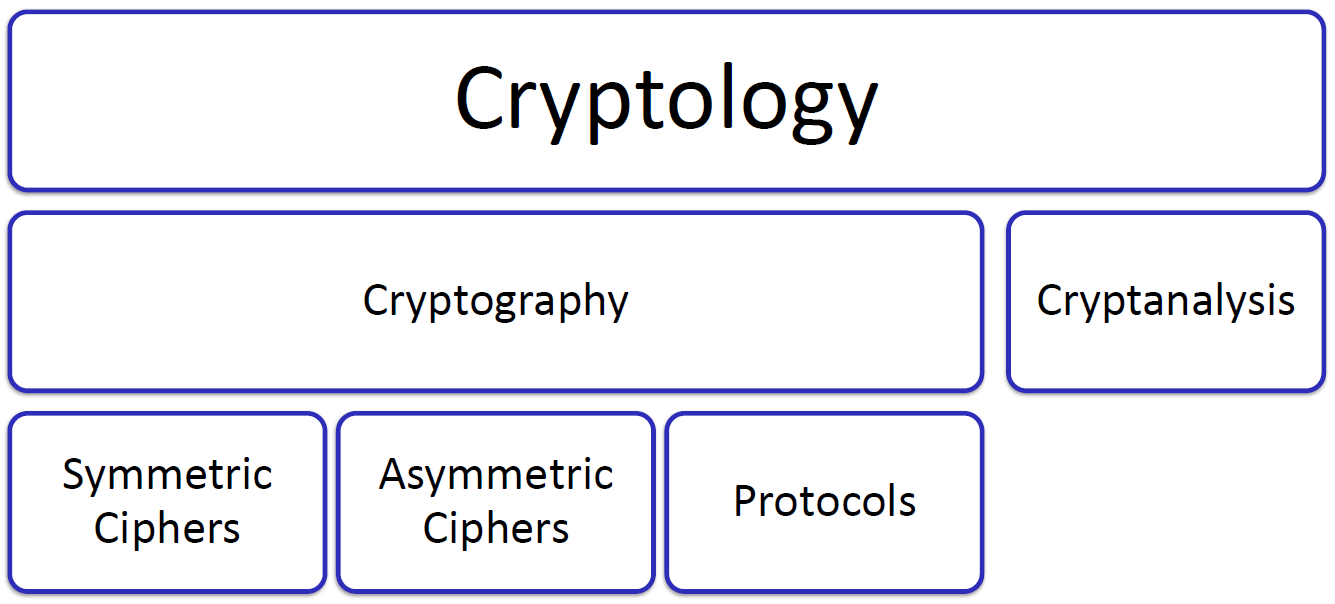
\includegraphics[width=0.5\linewidth]{images/EmbeddedSecurity/cryptologyOverview}

\textbf{Security through obscurity is no security at all}
\begin{itemize}
  \item No homebrew ciphers, no secret algorithms!
  \begin{itemize}
    \item The algorithm must not be secret
    \item The secrecy is in the keys, not in the algorithm (Kerckhoff's principle)
  \end{itemize}
  \item Breaking one device vs. breaking all devices
  \begin{itemize}
    \item Code is the same, keys are different
  \end{itemize}
  \item Real world analogy
  \begin{itemize}
    \item Attacker sees lock maker \& model
    \item Best option is brute force attack
  \end{itemize}
\end{itemize}

\subsection{Cryptography \& Random Numbers}
\begin{itemize}
  \item Many cryptographic operations require randomness
  \begin{itemize}
    \item Key generation
    \item Certain block cipher modes
    \item Secure protocols
  \end{itemize}
  \item But generating \& using random numbers is hard
  \begin{itemize}
    \item Computers are deterministic
    \item Estimating entropy is hard
  \end{itemize}
  \item PRNGs require a (truly) random seed, some usages don't seed at all(!!!)
  \item Use a CSPRNG (CS = Cryptographically Secure) if you have one
\end{itemize}
\textbf{Don't use C's rand() for anything security related!}

\subsection{Security Requirements}
\begin{description}
  \item[Confidentiality] (Vertraulichkeit)\\ Message can be understood only by the intended entities
  \item[Integrity] (Integrität)\\ Message is not altered/tampered by a third party
  \item[Authentication] (Authentisierung)\\ Ensures that the entities involved in an operation are who they claim to be
  \item[Non-Repudiation] (Nichtzurückweisbarkeit)\\ An entity cannot deny an action that it has performed
\end{description}

\subsubsection{Arrows in the quiver}
\begin{itemize}
  \item Secret key (symmetric) cryptography (AES, 3DES)
  \item Public key (asymmetric) cryptography
  \item Hashing
  \item \textbf{All secure data flows rely on more or less complex combinations of these algorithms}
\end{itemize}

\subsection{Secret key (symmetric) cryptography}

\begin{itemize}
  \item Very similar to lock \& key system
  \begin{itemize}
    \item Without the key, you can't get in
  \end{itemize}
  \item The lock is publicly viewable
  \begin{itemize}
    \item Key must remain with owner only
  \end{itemize}
  \item If the lock is weak, the key isn't necessary
  \begin{itemize}
    \item Same is true of a weak cipher
  \end{itemize}
  \item One key used to lock \& unlock the mechanism
  \begin{itemize}
    \item Symmetric crypto: same key used to encrypt and decrypt
  \end{itemize}
\end{itemize}
\begin{tabular}{|l|l|}
  \hline
  \textbf{Encryption:} & Ciphertext = Plaintext $\oplus$ Key\\
  \hline
  \textbf{Decryption:} & Plaintext = Ciphertext $\oplus$ Key\\
  \hline
\end{tabular}

\subsubsection{One Time Pad (OTP)}
Key: random string of bits, same length as plaintext
\begin{itemize}
  \item Impossible to crack when used correctly
\end{itemize}

Complications:
\begin{itemize}
  \item Generating true random numbers
  \begin{itemize}
    \item ''Bad'' random numbers are way too common
  \end{itemize}
  \item Never reuse the pad
  \begin{itemize}
    \item It's called ''one time'' for a reason
  \end{itemize}
  \item Key distribution
  \begin{itemize}
    \item Requires its own secure channel / method
  \end{itemize}
  \item Key synchronization
  \begin{itemize}
    \item Start at what character on what page of the pad?
  \end{itemize}
  \item Key disposal
\end{itemize}

\subsubsection{Alternatives to OTP}
\begin{itemize}
  \item Use shorter key
  \item Should be easier to handle
  \begin{itemize}
    \item Later: Key exchange with Asymmetric Cryptography
  \end{itemize}
  \item Goal:
  \begin{itemize}
    \item Change 1 bit of plaintext $\rightarrow$ Flip $\approx$ 50 \% of bits in ciphertext
  \end{itemize}
  \item Key length is relevant if best attack is brute force
  \begin{itemize}
    \item each additional bit doubles the effort
    \item Example AES: 128, 192, 256 bits
  \end{itemize}
  \item Old ciphers
  \begin{itemize}
    \item DES, 3DES
  \end{itemize}
  \item For today's use
  \begin{itemize}
    \item AES (Advanced Encryption Standard, Block Cipher)
  \end{itemize}
\end{itemize}

\subsubsection{Block Ciphers and their Modes}
\begin{minipage}{0.7\linewidth}
  \begin{itemize}
    \item AES block size: 128 bit
    \item How blocks of plaintext are processed
    \begin{itemize}
      \item Tradeoffs \& considerations
      \item We will look at several but not all modes
    \end{itemize}
    \item Initialization vectors
    \begin{itemize}
      \item Very important
      \item Typically required to be unique, sometimes also must be unpredictable
    \end{itemize}
    \item Padding
    \begin{itemize}
      \item Most of the time, (msgLen \% blockSize) != 0
      \item Padding correctly is very important
    \end{itemize}
  \end{itemize}
\end{minipage}
\begin{minipage}{0.3\linewidth}
  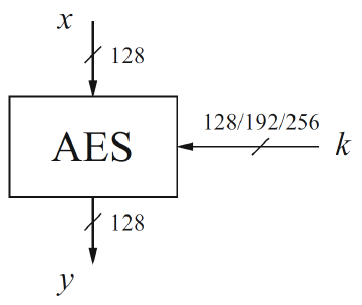
\includegraphics[width=\linewidth]{images/EmbeddedSecurity/aes}
\end{minipage}

\subsubsection{Electronic Codebook Mode (ECB)}
Don't use this mode\\
\begin{minipage}{0.6\linewidth}
  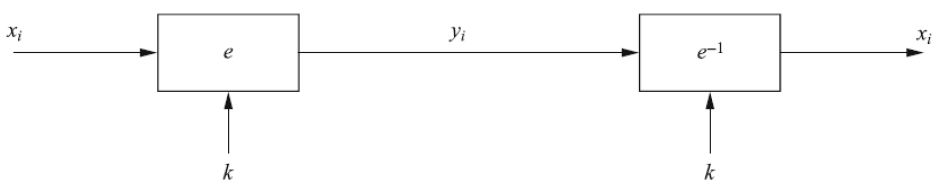
\includegraphics[width=0.8\linewidth]{images/EmbeddedSecurity/ecbBlock}
\end{minipage}
\begin{minipage}{0.4\linewidth}
  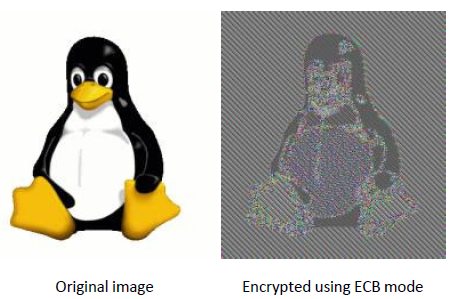
\includegraphics[width=0.9\linewidth]{images/EmbeddedSecurity/ecbImage}
\end{minipage}

\subsubsection{Cipher Block Chaining (CBC) Mode}
\begin{minipage}{0.3\linewidth}
\begin{itemize}
  \item Good mode
  \item IV (Initialization Vector) (aka Nonce: number only used once) must be set and unique, but may not be secret!
\end{itemize}
\end{minipage}
\begin{minipage}{0.7\linewidth}
  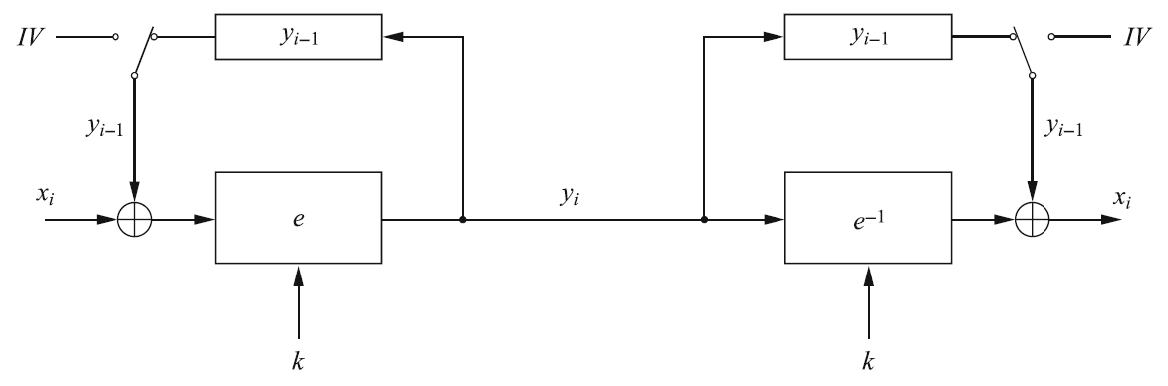
\includegraphics[width=\linewidth]{images/EmbeddedSecurity/cbcBlock}
\end{minipage}

\subsubsection{Counter (CTR) Mode}
\begin{minipage}{0.5\linewidth}
\begin{itemize}
  \item Good mode
  \item IV (Initialization Vector) (aka Nonce) must be set and unique, but may not be secret!
  \item Counter is incremented for each block
\end{itemize}
\end{minipage}
\begin{minipage}{0.5\linewidth}
  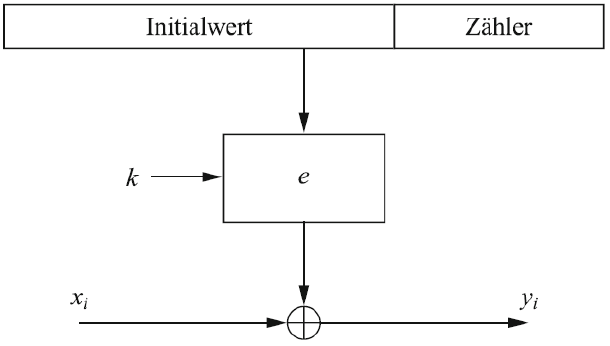
\includegraphics[width=\linewidth]{images/EmbeddedSecurity/ctrBlock}
\end{minipage}

\subsubsection{Which Cipher Mode Should I Use?}
\begin{itemize}
  \item Says Bruce Schneier:
  \begin{itemize}
    \item CBC with random IV
    \item Previously recommended CTR mode
  \end{itemize}
  \item Why the change?
  \begin{itemize}
    \item Too often, CTR's nonce was not unique
    \begin{itemize}
      \item Implementation issues (e.g. bugs) or deliberate attacks
    \end{itemize}
  \end{itemize}
\end{itemize}

\subsubsection{Authenticated Encryption Modes}
\textbf{Some modes provide authentication alongside secrecy}\\
Most common of these modes:
\begin{itemize}
  \item OCB (Offset Cookbook Mode)
  \begin{itemize}
    \item Essentially integrates a MAC into operation
    \item Doesn't require separate MAC \& encryption computations
    \item Covered by two patents (free license for OSS)
  \end{itemize}
  \item GCM (Galois Counter Mode), supported by STM32
  \begin{itemize}
    \item Combines CTR mode with Galois field multiplication
    \item Block sizes of 128, 192 and 256 bits
    \item Unencumbered by patents
  \end{itemize}
\end{itemize}

\subsubsection{Stream Cipher Basics}
\begin{itemize}
  \item Stram Ciphers generate a key stream
  \begin{itemize}
    \item Key stream used to encrypt plaintext\\
    Ciphertext = Plaintext $\oplus$ Key stream
  \end{itemize}
  \item Plaintext, Ciphertext and Key
  \begin{itemize}
    \item All the same length
    \item No padding required for stream cipher (it's not a block)
  \end{itemize}
  \item Security of system
  \begin{itemize}
    \item It's the key stream generator
    \item Output must be pseudorandom bit stream
  \end{itemize}
\end{itemize}

\subsubsection{Stream Cipher Inputs}
\begin{itemize}
  \item Key stream generator inputs
  \begin{itemize}
    \item Initialization Vector (IV), secret key
  \end{itemize}
  \item IV must be a nonce
  \begin{itemize}
    \item Number used once
    \item \textbf{Must be different each time}
    \item Otherwise identical key stream generated
  \end{itemize}
  \item IV doesn't need to be secret or random
  \begin{itemize}
    \item Generally transmitted in clear alongside ciphertext
    \item Needed by receiving party to generate same key
  \end{itemize}
\end{itemize}

\subsection{Public key (asymmetric) cryptography}

\subsubsection{Hashing}
\paragraph{Hash function}
\begin{itemize}
  \item Input: an arbitrarily long message (stream, file, etc.)
  \item Output: ''Digests'' input into a shorter, fixed-length representation
  \begin{itemize}
    \item The message's ''digital fingerprint''
  \end{itemize}
  \item Digest is not an encrypted form
  \item It's irreversible
  \begin{itemize}
    \item There are an infinite number of inputs for any given digest/output
  \end{itemize}
  \item But: it's very hard to manipulate the long message and still get the same digest
  \item Examples: MD5, SHA-1, SHA-2 (all supported by STM32)
\end{itemize}

\paragraph{Common uses of hash function}
\begin{itemize}
  \item Integrity Check
  \item File de-duplication
  \item Password storage \& verification
  \item Digital Signatures
  \item Message Authentication Codes
  \item Key derivation / generation from secret key
  \item Pseudo-Random Number Generation
  \item Proof of work (e.g. HashCash, Bitcoin)
\end{itemize}
